\documentclass[12pt]{book}
\usepackage[utf8]{inputenc}
\usepackage[T1]{fontenc}
\usepackage{mathptmx}
\usepackage{geometry}
\usepackage{mathtools}
\usepackage[english]{babel}
\usepackage{graphicx}
\usepackage{subcaption}
\usepackage{stackengine}
\usepackage[os=win]{menukeys}
\usepackage{hyperref}
\usepackage{minted}
\usepackage{xcolor}
\usepackage{tikz}
\usepackage[yyyymmdd,hhmmss]{datetime}
\usepackage{etoolbox}
\usepackage[inline]{enumitem}
\usepackage{pdfpages}

\newcommand{\WindowsLogo}{\raisebox{-0.1em}{\includegraphics[height=0.8em]{images/logo/Windows_3_logo_simplified}}}
%\newcommand{\PowerLogo}{\raisebox{-0.1em}{\includegraphics[height=0.8em]{images/logo/power}}}
\newcommand{\WinKey}{\keys{\WindowsLogo}}
\newcommand{\PowerKey}{\keys{\PowerLogo}}

\patchcmd{\thebibliography}{\section*{\refname}}{}{}{}

\newcommand{\ShowOsVersion}{
	\immediate\write18{\unexpanded{foo=`uname -sro` && echo "${foo}" > tmp.tex}}
	\input{tmp}\immediate\write18{rm tmp.tex}
}

\newcommand{\ShowTexVersion}{
	\immediate\write18{\unexpanded{foo=`pdflatex -version | head -n1 | cut -d' ' -f1,2` && echo "${foo}" > tmp.tex}}
	\input{tmp}\immediate\write18{rm tmp.tex}
}

\addto\captionsenglish{\renewcommand{\contentsname}{Daftar Isi}}
\addto\captionsenglish{\renewcommand{\figurename}{Gambar}}

\hypersetup{
	colorlinks=true, %set true if you want colored links
	linktoc=all,     %set to all if you want both sections and subsections linked
	linkcolor=blue,  %choose some color if you want links to stand out
	urlcolor=blue,   %url color
}

\geometry{
	a4paper,
	left=10mm,
	right=10mm,
	top=15mm,
	bottom=15mm,
}

\title{\LARGE \bf
	Pengenalan MathWorks MATLAB dan Pemrogramannya\\
}

\author{}

\date{}

\hypersetup{citecolor=black}

\definecolor{LightGray}{gray}{0.95}

%\pagecolor[rgb]{0.1,0.1,0.1}
%\color[rgb]{1,1,1}

\begin{document}
	\frontmatter
	\maketitle
	
	%%%%%%%%%%%%%%%%%%%%%%%%%%%%%%%%%%%%%%%%%%%%%%%%%%%%%%%%%%%%%%%%%
	
	\newpage
	\tableofcontents
	
	%%%%%%%%%%%%%%%%%%%%%%%%%%%%%%%%%%%%%%%%%%%%%%%%%%%%%%%%%%%%%%%%%
	
	\newpage
	\chapter{Disclaimer}
	
	MATLAB adalah merek dagang dari The MathWorks, Inc.
	The MathWorks sendiri tidak menjamin akurasi isi buku ini.
	Penggunaan buku dalam kaitan perangkat lunak MATLAB tidak bermaksud promosi atau sponsor dari MathWorks.
	\\
	\\
	Konten buku ini disarikan dari buku \textit{"Chemical Engineering Computation with MATLAB"} oleh Yeong Koo Yeo,
	dipublikasikan oleh CRC Press tahun 2001.
	
	%%%%%%%%%%%%%%%%%%%%%%%%%%%%%%%%%%%%%%%%%%%%%%%%%%%%%%%%%%%%%%%%%
	
	\newpage
	\chapter{Penggunaan Buku}
	
	\section{Umum}
	Buku ini dibuat dengan tujuan penggunaan utama sebagai panduan digital.
	Anda tidak perlu mencetak buku ini ke bentuk kertas.
	Seluruh navigasi buku ini diharapkan menggunakan klik ke hyperlink di Daftar Isi,
	atau menggunakan tampilan \textbf{Index} yang tersedia di \textbf{SideBar} program pembaca PDF yang anda gunakan.
	
	\section{Petunjuk}
	Beberapa petunjuk yang digunakan di buku ini:
	\begin{itemize}
		\item \textbf{Cetak Tebal}: Menginformasikan identifier (keyword, variabel, fungsi, alamat, nama file, dst) yang berada di suatu paragraf
		\item \textit{Cetak Miring}: Bersama simbol panah (->) dan simbol lain, menginformasikan langkah-langkah klik menu/tombol.
		\item \textbf{TIPS:} Menginformasikan hal-hal yang dapat membantu atau pengetahuan tambahan.
		\item \textbf{PERINGATAN:} Menginformasikan hal-hal yang bener-benar harus diperhatikan.
	\end{itemize}

	\section{Penulisan Kode} 
	Untuk penulisan kode, akan digunakan tiga bentuk:
	\begin{itemize}
		\item IN dan OUT. Berupa bagian kode, dengan:
		\begin{itemize}
			\item Baris dengan tanda \textbf{Prompt} (>>) adalah Input.
			Anda tidak perlu ketik ulang prompt.
			\item Baris dibawahnya tanpa ada tanda \textbf{Prompt} (>>) adalah contoh Output
		\end{itemize}
	
		\begin{minted}[frame=lines,framesep=2mm,fontsize=\small,bgcolor=LightGray]{matlab}
>> input
output
		\end{minted}
	
		\item IN saja. Hanya sebagai input dengan ditandai \textbf{Prompt} (>>).
		Anda tidak perlu ketik ulang prompt.
		Contoh Output disini tidak ditampilkan.
		
		\begin{minted}[frame=lines,framesep=2mm,fontsize=\small,bgcolor=LightGray]{matlab}
>> input
		\end{minted}
	
		\item Script/Function. Kode ditulis sebagai file script atau function tanpa ada tanda \textbf{Prompt} (>>) sama sekali.
		
		\begin{minted}[frame=lines,framesep=2mm,fontsize=\small,bgcolor=LightGray]{matlab}
function y=tambah(a,b)
	y = a + b
end
		\end{minted}
\end{itemize}
	
	%%%%%%%%%%%%%%%%%%%%%%%%%%%%%%%%%%%%%%%%%%%%%%%%%%%%%%%%%%%%%%%%%
	
	\newpage
	\mainmatter
	\chapter{Program MATLAB}
	
	Program MATLAB adalah program komputasi yang digunakan secara universal dalam bidang Sains dan Engineering.
	Secara garis besar, MATLAB adalah program kalkulator super canggih yang dapat menyelesaikan proses perhitungan kompleks.
	
	\section{Memulai Program}
	
	Anda dapat memulai program MATLAB sebagaimana program lainnya.
	
	\subsection{Windows}
	Untuk Windows 7, 8 , dan 10, Tekan tombol \textit{Start Windows} (\keys{\WindowsLogo}) dan ketik "MATLAB" untuk mencari program MATLAB yang terinstal.
	Tekan \textit{Enter} (\keys{\return}) untuk memulai
	\begin{figure}[!ht]
		\centering
		\includegraphics[width=250pt]{images/startmenuwin}
		\caption{Start MATLAB Windows}
	\end{figure}

	\subsection{GNU/Linux}
	Untuk GNU/Linux seperti ArchLinux, Manjaro, atau Ubuntu, tekan \textit{Start Menu} -> MATLAB.
	\begin{figure}[!ht]
		\centering
		\includegraphics[width=200pt]{images/startmenumate}
		\caption{Start MATLAB GNU/Linux}
	\end{figure}

	\newpage
	Metode lainnya adalah memanggil program matlab dengan Terminal/Bash Emulator dan masukkan perintah:
	\begin{minted}[frame=lines,framesep=2mm,fontsize=\small,bgcolor=LightGray]{bash}
$> matlab
	\end{minted}
	
	\subsection{MacOS}
	
	Menyusul
	
	\newpage
	\section{Bagian Antar Muka}
	
	Antar Muka (Interface) program MATLAB dapat berbeda antara satu pengguna dan pengguna lainnya.
	Berikut salah satu tampilan default yang umum dipakai:
	
	\begin{figure}[!ht]
		\centering
		\begin{subfigure}[b]{0.75\textwidth}
			\includegraphics[width=\textwidth]{images/matlabiface}
		\end{subfigure}
		\begin{subfigure}[b]{0.2\textwidth}
			\includegraphics[width=\textwidth]{images/matlabpart}
		\end{subfigure}
		\caption{Bagian Antar Muka}
	\end{figure}
	
	\subsection{Default Layout}
	
	Jika ingin untuk mengembalikan penataan (Layout) antar muka program, anda dapat melakukannya melalui Toolbar.
	Pilih tab \textit{Home} -> \textit{Layout}, kemudian pilih \textit{Default} atau \textit{Two-Column}.
	
	\begin{figure}[!ht]
		\centering
		\includegraphics[width=150pt]{images/matlablayout}
		\caption{Penataan MATLAB}
	\end{figure}
	
	\subsection{Toolbar}
	Toolbar disini bertindak sama seperti Toolbar pada Microsoft Office.
	Disini tersedia beragam perintah dalam bentuk icon yang dapat diklik.
	
	\newpage
	Tab yang tersedia antara lain:
	\begin{itemize}
		\item \textit{Home}. Berisi perintah dasar untuk mengolah file, variable, pengaturan program, dan layout.
		\item \textit{Plot}. Berisi perintah pengolahan plot langsung dari variable yang tersedia di Workspace.
		\item \textit{Apps}. Berisi perintah tambahan dari toolbox atau addon yang terinstal.
		\item \textit{Editor}. Berisi perintah untuk mengolah file, mengelola jalannya suatu skrip, dan perintah editing.
		Hanya muncul jika Editor diaktifkan.
		\item \textit{Publish}. Berisi perintah untuk membantu publikasi dan berbagi kode sumber melalui website MATLAB.
		Hanya muncul jika Editor diaktifkan.
		\item \textit{View}. Berisi perintah untuk mengolah tampilan kode sumber yang sedang diedit.
		Hanya muncul jika Editor diaktifkan.	
	\end{itemize}

	\subsection{Current Address}
	
	Current Address digunakan untuk menunjukkan alamat folder yang sedang aktif dan membantu navigasi berpindah folder.
	Icon tersedia antara lain panah navigasi (seperti pada webbrowser), icon folder untuk jelajah folder dengan program \textit{file-manager},
	teks alamat folder yang dapat diedit, icon panah bawah untuk history, dan icon lup untuk mencari.
	
	Untuk berpindah folder, anda dapat input teks alamat folder secara manual.
	Anda cukup klik alamat dan saat muncul cursor, anda dapat edit/paste alamat dan kemudian tekan Enter (\keys{\return}) untuk berpindah folder.
	
	\begin{figure}[!ht]
		\centering
		\includegraphics[width=350pt]{images/addressbaredit}
		\caption{Pindah Alamat}
	\end{figure}

	\textbf{TIPS:} Alamat di atas adalah format alamat untuk Unix (Linux/MacOS).
	Untuk Windows, alamat akan memiliki format dimulai "\textbf{C:\textbackslash}" atau "\textbf{D:\textbackslash}" sesuai drive.
	
	Selain itu, anda juga dapat menggunakan history untuk berpindah folder.
	Tekan icon panah bawah di sisi kanan alamat.
	
	\begin{figure}[!ht]
		\centering
		\includegraphics[width=350pt]{images/addressbarhistory}
		\caption{History Alamat}
	\end{figure}
	
	\newpage
	\subsection{Current Folder}
	
	Current Folder menampilkan file dan folder di alamat yang sedang aktif.
	Anda dapat membuka, menghapus, membuat, dan memindahkan file disini.
	Anda juga dapat berpindah folder dengan double-klik folder yang tersedia.
	
	\begin{figure}[!ht]
		\centering
		\includegraphics[width=150pt]{images/currentfolder}
		\caption{Current Folder}
	\end{figure}

	\subsection{Command Window}
	
	Command Window adalah bagian utama MATLAB dimana anda memasukkan perintah-perintah teks untuk diproses oleh MATLAB.
	Hasil proses juga akan ditampilkan disini.
	
	\begin{figure}[!ht]
		\centering
		\includegraphics[width=250pt]{images/commandwindow}
		\caption{Command Window}
	\end{figure}

	sebagai percobaan, coba masukkan perintah berikut dan tekan ENTER (\keys{\return})
	
	\begin{minted}[frame=lines,framesep=2mm,fontsize=\small,bgcolor=LightGray]{matlab}
>> a = 10^2
a = 
   100
	\end{minted}
	
	\subsubsection{TIPS:}
	
	Berikut beberapa tips yang sangat membantu:
	
	\begin{itemize}
		\item \textbf{Tanda Prompt}
		
		Prompt digunakan sebagai penanda baris dimana anda dapat memasukkan perintah ke MATLAB.
		Tanda prompt berupa dua panah ke kanan (\textbf{>>}) di Command Window.
		
		\item \textbf{Menghentikan Proses}
		
		Apabila terjadi ingin menghentikan suatu proses eksekusi perintah,
		anda dapat menggunakan kombinasi tombol CTRL+c (menekan tombol \keys{Ctrl} dan huruf \keys{c} bersamaan di keyboard).
	
		Sebagai contoh, masukkan perintah berikut:
		\begin{minted}[frame=lines,framesep=2mm,fontsize=\small,bgcolor=LightGray]{matlab}
>> while(true);pause(1);end
		\end{minted}
		
		Disini terlihat ada jarak satu baris namun tidak ada tanda Prompt,
		menandakan MATLAB sedang sibuk dan tidak dapat menerima perintah lebih lanjut.
		
		Untuk menghentikan proses, tekan \keys{Ctrl} dan huruf \keys{c} bersamaan.
		
		\item \textbf{Semi-Colon}
		
		Tanda Semi-Colon (\keys{;}), memiliki 2 fungsi:
		\begin{enumerate}
			\item Sebagai pemisah statement untuk satu baris.
			Sebagai contoh berikut deklarasikan 3 variable.
			\begin{minted}[frame=lines,framesep=2mm,fontsize=\small,bgcolor=LightGray]{matlab}
>> varA = 10
>> varB = 20
>> varC = 30
			\end{minted}
		
			Anda juga dapat menuliskannya sebagai:
			\begin{minted}[frame=lines,framesep=2mm,fontsize=\small,bgcolor=LightGray]{matlab}
>> varA = 10; varB = 20; varC = 30
			\end{minted}
		
			\item Untuk menyembunyikan (suppress) respon output untuk perintah yang dijalankan
			Sebagai contoh perintah berikut:
			\begin{minted}[frame=lines,framesep=2mm,fontsize=\small,bgcolor=LightGray]{matlab}
>> varA = 10
varA =
	10
			\end{minted}
		
			Terlihat bahwa MATLAB akan merespon memberitahukan bahwa varA bernilai 10.
			Jika perintah di atas diakhiri tanda semi-colon (\keys{;}):
			
			\begin{minted}[frame=lines,framesep=2mm,fontsize=\small,bgcolor=LightGray]{matlab}
>> varA = 10;
			\end{minted}
		
			maka MATLAB tidak akan menampilkan respon apa pun saat eksekusi sukses.
		\end{enumerate}
	
		\item \textbf{Pembersihan}
		
		Untuk membersihkan Command Window, masukkan perintah berikut:
		\begin{minted}[frame=lines,framesep=2mm,fontsize=\small,bgcolor=LightGray]{matlab}
>> clc
		\end{minted}
	
		\textbf{PERINGATAN:} Membersihkan Command Window \textbf{tidak} otomatis membersihkan variable yang tersimpan di memory MATLAB.
	
		\newpage
		\item \textbf{Sugesti}
		
		Untuk mempercepat input perintah, tersedia fitur Sugesti atau Auto-complete.
		Sebagai contoh, masukkan kata \textbf{pow} di Command Window, kemudian tekan tombol (\keys{Tab}).
		
		\begin{figure}[!ht]
			\centering
			\includegraphics[width=100pt]{images/commandtab}
			\caption{Command Window Sugesti}
		\end{figure}
	
		Silahkan pilih dengan tombol \keys{$\uparrow$} dan \keys{$\downarrow$}.
		Tekan ENTER (\keys{\return}) untuk eksekusi pilihan.
		
		\item \textbf{History}.
		Jika ingin mengulang perintah yang sama atau telah dimasukkan sebelumnya,
		ada cukup klik dekat dekat tanda Prompt di Command Window, kemudian tekan tombol panah atas (\keys{$\uparrow$})
		
		\begin{figure}[!ht]
			\centering
			\includegraphics[width=200pt]{images/commandhistory}
			\caption{Command Window History}
		\end{figure}
		
		Akan muncul history perintah yang pernah dimasukkan.
		Anda tinggal pilih dengan tombol panah atas (\keys{$\uparrow$}) dan panah bawah (\keys{$\downarrow$}).
		Tekan ENTER (\keys{\return}) untuk mengeksekusi perintah yang dipilih.
		
	\end{itemize}
	
	\subsection{Ready Indicator}
	
	Bagian ini menunjukkan siap tidaknya MATLAB untuk menerima perintah.
	Kemungkinan nilai yang muncul:
	\begin{itemize}
		\item \textbf{Busy}. Menandakan MATLAB sedang sibuk dan tidak bisa menerima perintah.
		\item \textbf{Ready}. Menandakan MATLAB siap menerima perintah setelah start-up.
		\item \textbf{Tidak ada label}. Menandakan MATLAB siap menerima perintah.
	\end{itemize}
	
	\subsection{Workspace}
	
	Workspace adalah tempat semua variable yang bersifat global ditampilkan.
	Disini kita dapat melihat nilai suatu variable, ukuran dan nilai array, serta variable yang di-import.
	
	Sebagai contoh jika kita masukkan perintah:
	\begin{minted}[frame=lines,framesep=2mm,fontsize=\small,bgcolor=LightGray]{matlab}
>> varA = 10; varB = 20; varC = 30
	\end{minted}

	\newpage
	Maka tampil di Workspace:
	
	\begin{figure}[!ht]
		\centering
		\includegraphics[width=150pt]{images/workspace}
		\caption{Variabel di Workspace}
	\end{figure}

	Untuk membersihkan Workspace, masukkan perintah berikut di Command Window
	\begin{minted}[frame=lines,framesep=2mm,fontsize=\small,bgcolor=LightGray]{matlab}
>> clear
	\end{minted}
		
	\subsection{Editor}
	Editor adalah bagian MATLAB yang digunakan untuk menulisan skrip yang dapat dieksekusi oleh MATLAB.
	Skrip pada dasarnya adalah kumpulan perintah-perintah MATLAB (dapat dieksekusi di Command Window),
	yang kemudian dieksekusi secara berurutan dari baris atas ke bawah dari file skrip.
	
	Sebagai contoh, masukkan perintah-perintah berikut ke Editor (bukan Command-Window)
	\begin{minted}[frame=lines,framesep=2mm,fontsize=\small,bgcolor=LightGray]{matlab}
clear;
clc;

varA = 10;
varB = 20;
varC = 30;
	\end{minted}

	Klik icon \textit{Save} pada toolbar tab \textit{Editor} dengan nama file berektensi \textbf{*.m}.
	
	\begin{figure}[!ht]
		\centering
		\includegraphics[width=175pt]{images/editorcoba}
		\caption{Contoh Skrip pada Editor}
	\end{figure}
	
	Selanjutnya, klik icon \textit{Run} (panah segitiga hijau) pada toolbar tab \textit{Editor} untuk menjalankan skrip.
	
	Atau dapat pula dipanggil melalui Command Window dengan memasukkan nama file skrip tanpa ekstensi.
	Contoh jika skrip disimpan sebagai \textbf{coba.m}, maka perintah untuk memanggil skrip:
	\begin{minted}[frame=lines,framesep=2mm,fontsize=\small,bgcolor=LightGray]{matlab}
>> coba
	\end{minted}
	
	\textbf{TIPS:} Topik file skrip dan file fungsi lebih jauh akan dibahas pada bab selanjutnya. 
	
	\newpage
	\chapter{Pemrograman Dasar}
	
	Bab ini menjelaskan tutorial pemrograman dasar MATLAB.
	Untuk dapat mengikuti panduan ini, diasumsikan bahwa telah familiar dengan antar-muka MATLAB sebagaimana dijelaskan bab sebelumnya.
	Terutama bagian Command-Window karena panduan ini akan berfokus menggunakan Command-Window.
	
	\section{Operator}
	
	\subsection{Matematika Dasar}
	
	Berikut operator dasar matematika:
	
	\begin{center}
		\begin{tabular}{|c|c|}
			\hline
			Operator & Makna \\
			\hline\hline
			+ & Penambahan \\
			\hline
			- & Pengurangan \\
			\hline
			* & Perkalian \\
			\hline
			/ & Pembagian \\
			\hline
			\char`\^ & Pangkat \\
			\hline
		\end{tabular}
	\end{center}

	\textbf{PERHATIAN:} Simbol "\textbf{/}" (pembagi) dan "\textbf{\textbackslash}" (linear solver) memiliki makna yang jauh berbeda.
	Harap diperhatikan.
	
	Contoh:
	\begin{minted}[frame=lines,framesep=2mm,fontsize=\small,bgcolor=LightGray]{matlab}
>> 10^2
ans = 
    100
	\end{minted}
	
	\textbf{TIPS:} variable \textbf{ans} (singkatan dari answer), adalah variabel output default jika tidak ada assigment variable dalam statement.
	Anda dapat menggunakan variable \textbf{ans} untuk operasi selanjutnya
	
	Contoh:
	\begin{minted}[frame=lines,framesep=2mm,fontsize=\small,bgcolor=LightGray]{matlab}
>> 10^2
ans = 
    100
	
>> ans^2
ans = 
    10000
	\end{minted}

	Untuk urutan operasi dalam satu baris, tetap mengikuti kaidah priotias dimana operasi pangkat didahulukan, diikuti perkalian dan pembagian, kemudian tambah dan kurang.
	Namun urutan ini juga dapat di override menggunakan tanda kurung.
	
	Contoh:
	\begin{minted}[frame=lines,framesep=2mm,fontsize=\small,bgcolor=LightGray]{matlab}
>> 8+2^2
ans = 
    12

>> 8+4*2^2
ans = 
    24
	
>> (8+2)^2
ans =
    100
	\end{minted}

	Sedangkan untuk operasi di luar perhitungan aritmatik (semisal trigonometri, logaritma, sisa pembagian, akar, dst), tidak menggunakan operator khusus.
	Melainkan menggunakan fungsi-fungsi yang tersedia di MATLAB.
	
	Contoh Trigonometri (Radiant):
	\begin{minted}[frame=lines,framesep=2mm,fontsize=\small,bgcolor=LightGray]{matlab}
>> sin(0.5*pi)
ans = 
    1
    
>> tan(0.5*pi)
ans = 
    1.6331e+16
	\end{minted}

	\textbf{TIPS:} Notasi angka dengan \textbf{A.BBe+C} atau \textbf{A.BBe-C} adalah bentuk notasi saintifik.
	Equivalen dengan bentuk $A.BB x 10^C$ atau $A.BB x 10^{-C}$.
	Untuk contoh fungsi \textbf{tan()} di atas, notasi saintifik hasilnya adalah (\textbf{$1.6331x10^{16}$}).
	\\
	\\
	\textbf{TIPS:} Implementasi Trigonometri di MATLAB pada dasarnya menggunakan pendekatan deret.
	Untuk itu, beberapa fungsi seperti \textbf{tan(pi/2)} seperti di atas memberikan nilai yang sangat besar (mencapai $10^{16}$)
	alih-alih nilai tak berhingga sebagaimana kaidah umum Trigonometry.
	
	\subsection{Variabel Dasar}
	
	Variabel adalah identifier dalam pemrograman yang digunakan untuk menyimpan suatu nilai.
	Seluruh pengolahan dan perhitungan dalam MATLAB umumnya dilakukan pada variabel.
	
	Untuk membuat variable, anda cukup melakukan assignment:
	\begin{minted}[frame=lines,framesep=2mm,fontsize=\small,bgcolor=LightGray]{matlab}
>> varA = 10;
	\end{minted}

	Anda juga dapat membuat variable dari hasil fungsi atau perhitungan
	\begin{minted}[frame=lines,framesep=2mm,fontsize=\small,bgcolor=LightGray]{matlab}
>> varB = 8^2;
>> varC = sin(pi/2);
	\end{minted}

	Variable yang ada buat akan tampil di Workspace, atau dapat dilihat dengan perintah:
	\begin{minted}[frame=lines,framesep=2mm,fontsize=\small,bgcolor=LightGray]{matlab}
>> who
	\end{minted}

	\newpage
	Anda dapat melihat isi variable dengan memanggil nama variabel tersebut
	\begin{minted}[frame=lines,framesep=2mm,fontsize=\small,bgcolor=LightGray]{matlab}
>> varA
varA =
     10
	\end{minted}

	Dengan konsep variabel, anda dapat melakukan kalkulasi dengan nilai yang berubah-ubah sesuai proses kalkulasi namun dengan nama identifier tetap.
	\begin{minted}[frame=lines,framesep=2mm,fontsize=\small,bgcolor=LightGray]{matlab}
>> varA = varB + varC
varA =
     65
	\end{minted}

	\textbf{PERHATIAN:} Beberapa aturan dalam membuat nama variabel atau fungsi:
	\begin{itemize}
		\item Terdiri dari kombinasi alphanumeric (a-z, A-Z, dan 0-9) dan underscore (\_)
		\item Karakter pertama hanya boleh huruf, tidak boleh angka dan tidak boleh underscore.
		\item Tidak boleh memakai titik (\textbf{.}) karena simbol titik adalah operator yang memiliki arti sendiri (untuk data struktur)
		\item Tidak boleh memakai spasi karena spasi adalah pemisah identifier.
		Jika butuh dua kata untuk nama variable, dapat menggunakan:
		\begin{enumerate}
			\item pemisah undescore (\_), contoh: var\_Baru, var\_Lama, dst
			\item camel-case, contoh: varBaru, varLama
		\end{enumerate}
		\item Gunakan nama variabel yang ringkas dan mudah diingat.
	\end{itemize}
	
	\subsection{Operasi Logika}
	
	Berikut adalah pembahasan operator logika dimana kalkulasi dilakukan ke variable boolean.
	Variable Boolean adalah variable yang hanya memiliki nilai benar (\textbf{true}) atau salah (\textbf{false}).
	Nilai \textbf{true} setara dengan nilai 1 dan \textbf{false} setara dengan 0.
	Operasi Logika akan sangat bermanfaat nanti untuk topik kendali \textbf{if} dan perulangan \textbf{loop}.
	
	\begin{itemize}
		\item \textbf{not (\textasciitilde)}. Untuk membalik atau negasi nilai boolean.
		\begin{minted}[frame=lines,framesep=2mm,fontsize=\small,bgcolor=LightGray]{matlab}
>> A = true
A =
  1
  
>> ~A
ans =
   0
   
>> not(A)
ans =
   0 
		\end{minted}
		
		\newpage
		\item \textbf{and (\&)}. Untuk membandingkan dua nilai boolean dimana akan bernilai benar jika keduanya benar.
		\begin{minted}[frame=lines,framesep=2mm,fontsize=\small,bgcolor=LightGray]{matlab}
>> A = true; B = true;
>> A & B
ans = 
    1

>> and(A,B)
ans = 
    1
    
>> and(A, ~B)
ans = 
    0
		\end{minted}
		
		\item \textbf{or (|)}. Untuk membandingkan dua nilai boolean dimana akan bernilai benar jika salah satu benar.
		\begin{minted}[frame=lines,framesep=2mm,fontsize=\small,bgcolor=LightGray]{matlab}
>> A = true; B = true;
>> A | B
ans = 
    1

>> or(A,B)
ans = 
    1

>> or(A, ~B)
ans = 
    1
		\end{minted}
	\end{itemize}

	\section{Vektor/Matrix}
	
	\subsection{Vektor}
	\subsubsection{Membuat Vektor}
	\subsubsection{Index Vektor}
	
	\subsection{Matrix}
	\subsubsection{Membuat Matrix}
	\subsubsection{Index Matrix}
	
	\subsection{Operasi Vektor/Matrix}
	
	\section{Kendali Program}
	
	\subsection{Kondisi IF}
	\subsection{Kondisi SWITCH}
	\subsection{Loop WHILE}
	\subsection{Loop FOR}	
\end{document}